%%%%%%%%%%%%%%%%%%%%%%%%%%%%%%%%%%%%%%%%%
% Beamer Presentation
% LaTeX Template
% Version 1.0 (10/11/12)
%
% This template has been downloaded from:
% http://www.LaTeXTemplates.com
%
% License:
% CC BY-NC-SA 3.0 (http://creativecommons.org/licenses/by-nc-sa/3.0/)
%
%%%%%%%%%%%%%%%%%%%%%%%%%%%%%%%%%%%%%%%%%

%----------------------------------------------------------------------------------------
%	PACKAGES AND THEMES
%----------------------------------------------------------------------------------------

\documentclass{beamer}

\mode<presentation> {
	
	% The Beamer class comes with a number of default slide themes
	% which change the colors and layouts of slides. Below this is a list
	% of all the themes, uncomment each in turn to see what they look like.
	
	%\usetheme{default}
	%\usetheme{AnnArbor}
	%\usetheme{Antibes}
	%\usetheme{Bergen}
	%\usetheme{Berkeley}
	%\usetheme{Berlin}
	%\usetheme{Boadilla}
	%\usetheme{CambridgeUS}
	%\usetheme{Copenhagen}
	%\usetheme{Darmstadt}
	%\usetheme{Dresden}
	%\usetheme{Frankfurt}
	%\usetheme{Goettingen}
	%\usetheme{Hannover}
	%\usetheme{Ilmenau}
	%\usetheme{JuanLesPins}
	%\usetheme{Luebeck}
	\usetheme{Madrid}
	%\usetheme{Malmoe}
	%\usetheme{Marburg}
	%\usetheme{Montpellier}
	%\usetheme{PaloAlto}
	%\usetheme{Pittsburgh}
	%\usetheme{Rochester}
	%\usetheme{Singapore}
	%\usetheme{Szeged}
	%\usetheme{Warsaw}
	
	% As well as themes, the Beamer class has a number of color themes
	% for any slide theme. Uncomment each of these in turn to see how it
	% changes the colors of your current slide theme.
	
	%\usecolortheme{albatross}
	\usecolortheme{beaver}
	%\usecolortheme{beetle}
	%\usecolortheme{crane}
	%\usecolortheme{dolphin}
	%\usecolortheme{dove}
	%\usecolortheme{fly}
	%\usecolortheme{lily}
	%\usecolortheme{orchid}
	%\usecolortheme{rose}
	%\usecolortheme{seagull}
	%\usecolortheme{seahorse}
	%\usecolortheme{whale}
	%\usecolortheme{wolverine}
	
	%\setbeamertemplate{footline} % To remove the footer line in all slides uncomment this line
	%\setbeamertemplate{footline}[page number] % To replace the footer line in all slides with a simple slide count uncomment this line
	
	%\setbeamertemplate{navigation symbols}{} % To remove the navigation symbols from the bottom of all slides uncomment this line
}

\usepackage{graphicx} % Allows including images
\usepackage{subfigure}
\usepackage{booktabs} % Allows the use of \toprule, \midrule and \bottomrule in tables
\usepackage{bm}

%----------------------------------------------------------------------------------------
%	TITLE PAGE
%----------------------------------------------------------------------------------------

\title[Asymptotic LASSO]{Asymptotics for LASSO-type Estimators} 

\author{Ganchao Wei} 
\date{December 8, 2021}

\begin{document}
	
	\begin{frame}
		\titlepage % Print the title page as the first slide
	\end{frame}
	
	\begin{frame}
		\frametitle{Overview} % Table of contents slide, comment this block out to remove it
		\tableofcontents
	\end{frame}
	
	%--------------------------------------------------------------------
	%	PRESENTATION SLIDES
	%--------------------------------------------------------------------
	
	\section{Introduction}
	
	\begin{frame}
		\frametitle{Introduction}
		Consider the linear regression model:
		$$Y_i = \beta_0 + \bm{x}_i^T\bm{\beta} + \epsilon_i$$
		We estimate $\bm{\beta}$ by minimizing the penalized least squares criterion:
		$$\sum_{i=1}^{n}(Y_i-\bm{x}_i^T\bm{\phi})^2 + \lambda_n\sum_{j=1}^{p}|\phi_j|^{\gamma}$$
		Such estimators were called Bridge estimators.
		When $\lambda_n = 0$, it corresponds to the OLS estimator, denoted by $\hat{\bm{\beta}}_n^{(0)}$.
		
		Some special cases:
		\begin{itemize}
			\item
			 $\gamma = 2$, ridge regression
			 \item
			 $\gamma = 1$, LASSO regression
			 \item
			 $\gamma \to 0$, penalize by the number of nonzero parameters, e.g. AIC \& BIC.
		\end{itemize}
	\end{frame}
	
	\begin{frame}
		\frametitle{Introduction}
		Regularity conditions:
		\begin{itemize}
			\item 
			$C_n = \frac{1}{n}\sum_{i=1}^{n}\bm{x}_i^T\bm{x}_i \to C$
			\item
			$C_n$ is not singular (although this can be relaxed by equivalence class)
			\item
			First assume $C$ is nonsingular. It will be further relaxed when discussing "nearly singular" design.
			\item
			$\frac{1}{n}\max_{1\leq i \leq n}\bm{x}_i^T\bm{x}_i \to 0$
		\end{itemize}
		 Under the regularity conditions, we know the OLS estimator is consistent and:
		$$\sqrt{n}(\hat{\bm{\beta}}_n^{(0)} - \bm{\beta}) \to_{d} N(\bm{0}, \sigma^2C^{-1})$$
	\end{frame}
	
	\begin{frame}
		\frametitle{Limiting distributions}
		Assume $C$ is nonsingular. Define the (random) function:
		$$Z_n(\bm{\phi}) = \frac{1}{n}\sum_{i=1}^{n}(Y_i-\bm{x}_i^T\bm{\phi})^2 + \frac{\lambda_n}{n}\sum_{j=1}^{p}|\phi_j|^{\gamma}$$
		, which is minimized at $\bm{\phi} = \hat{\bm{\beta}}_n$. The following result shows that $\hat{\bm{\beta}}_n$ is consistent provided $\lambda_n = o(n)$
		\begin{figure}
			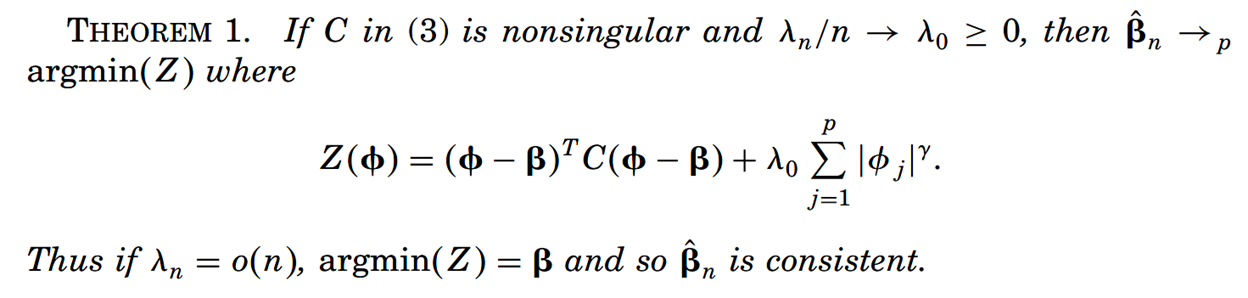
\includegraphics[width=1\linewidth]{image001.png}
		\end{figure}
	\end{frame}
	
	\begin{frame}
		\frametitle{Limiting distributions}
		Although $\lambda_n = o(n)$ is sufficient for consistency, we require that $\lambda_n$ grow slowly for $\sqrt{n}$-consistency, but not too small to reduce to OLS.
		
		For $\gamma \geq 1$, we need $\lambda_n = O(\sqrt{n})$
		\begin{figure}
			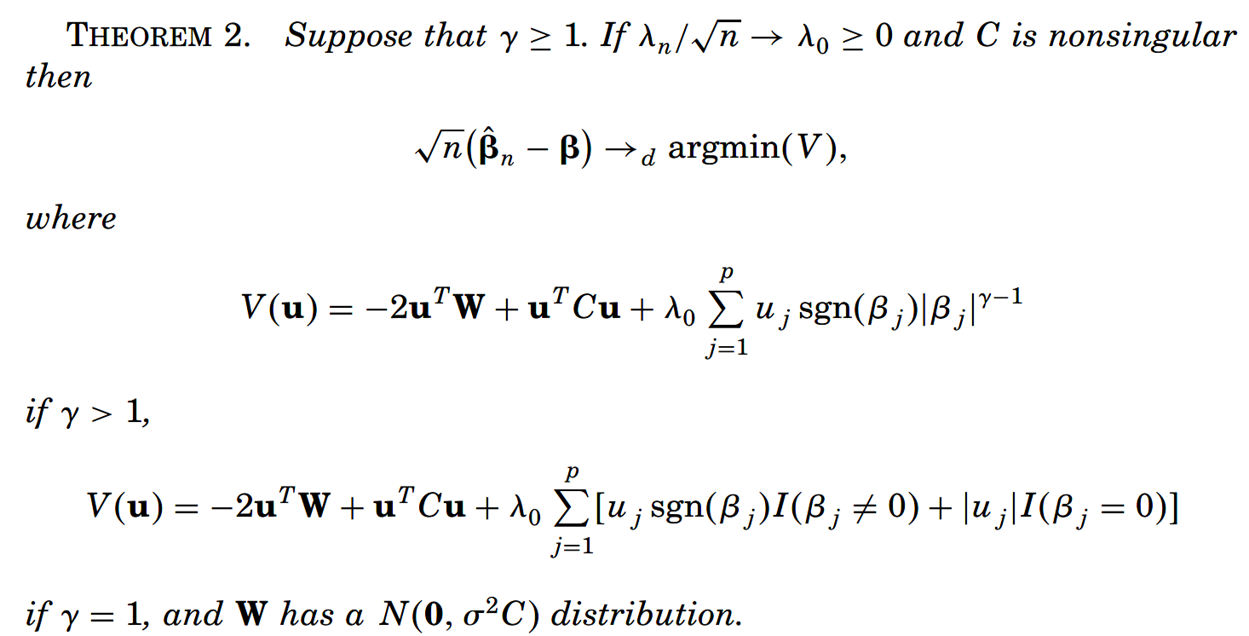
\includegraphics[width=1\linewidth]{image002.png}
		\end{figure}
	\end{frame}
	
	\begin{frame}
		\frametitle{Limiting distributions}
		Although $\lambda_n = O(\sqrt{n})$ suffices for $\gamma < 1$, we further suggests $\lambda_n = O(n^{\gamma/2})$ for $\gamma < 1$
		\begin{figure}
			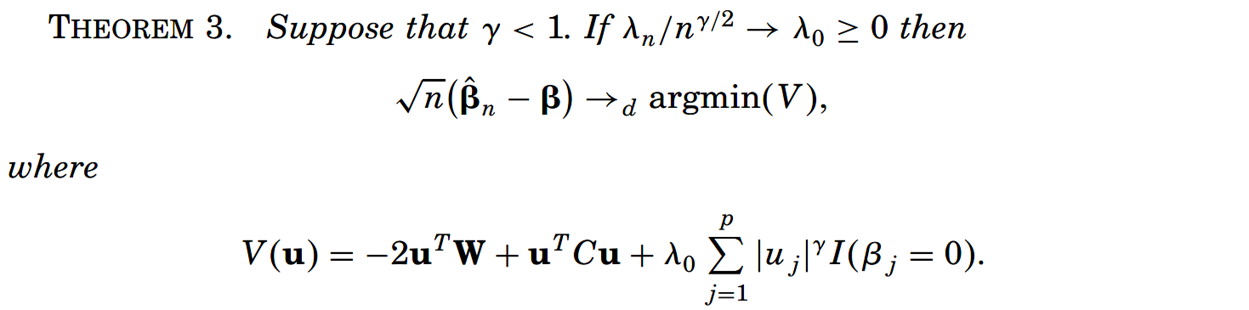
\includegraphics[width=1\linewidth]{image003.png}
		\end{figure}
		This is interesting:
		\begin{itemize}
			\item 
			Estimate nonzero regression parameters at the usual rate, without asymptotic bias
			\item
			Shrink the estimates of  zeros regression parameters to 0, with positive probability
			\item
			This is in contrast to theorem 2 ($\gamma \geq 1$): bias is $\lambda_0 > 0$
		\end{itemize}
	\end{frame}
	
	\begin{frame}
		\frametitle{Limiting distributions}
		In the following example, $\beta_1 > 0$ and $\beta_2 = 0$
		\begin{figure}
			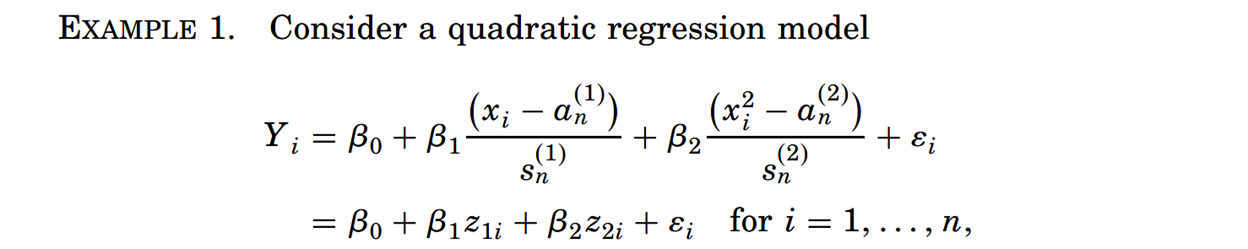
\includegraphics[width=1\linewidth]{image004.png}
		\end{figure}
	\end{frame}
	
	\begin{frame}
		\frametitle{Limiting distributions}
		\begin{figure}
			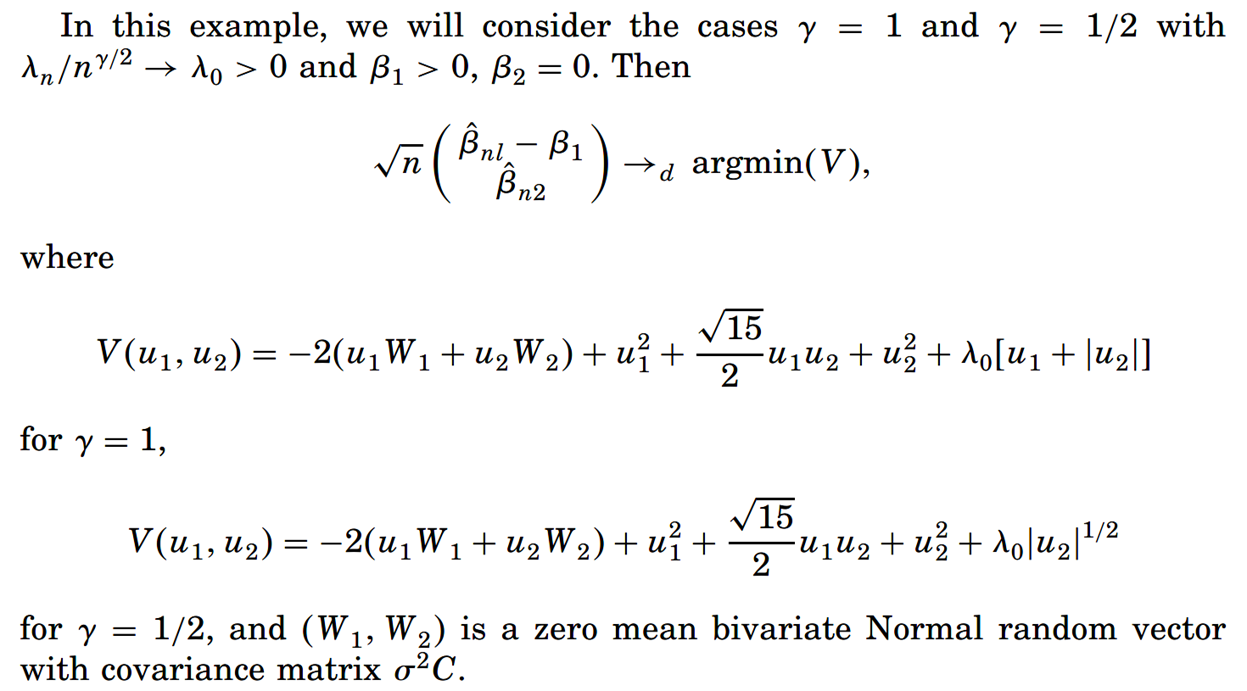
\includegraphics[width=1\linewidth]{image005.png}
		\end{figure}
	\end{frame}
	
	\begin{frame}
		\frametitle{Limiting distributions}
		For $\gamma = 1$:
		\begin{itemize}
			\item 
			the asymptotic variances decreases as $\gamma_0$ increases.
			\item
			As $\gamma_0$ increases, the asymptotic bias of $\hat{\beta}_{n1}$ becomes increasingly negative, while $\hat{\beta}_{n2}$ increase away from 0 then decreases to 0.
		\end{itemize}
		\begin{figure}
			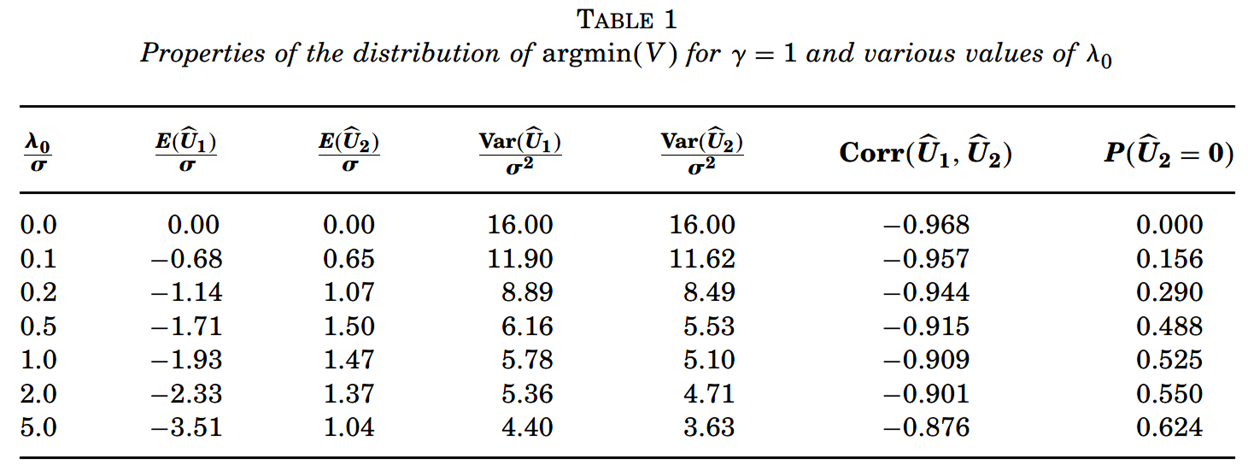
\includegraphics[width=1\linewidth]{image006.png}
		\end{figure}
	\end{frame}
	
	\begin{frame}
		\frametitle{Limiting distributions}
		But for $\gamma = 0.5$, things are different (in terms of the asymptotic bias):
		\begin{figure}
			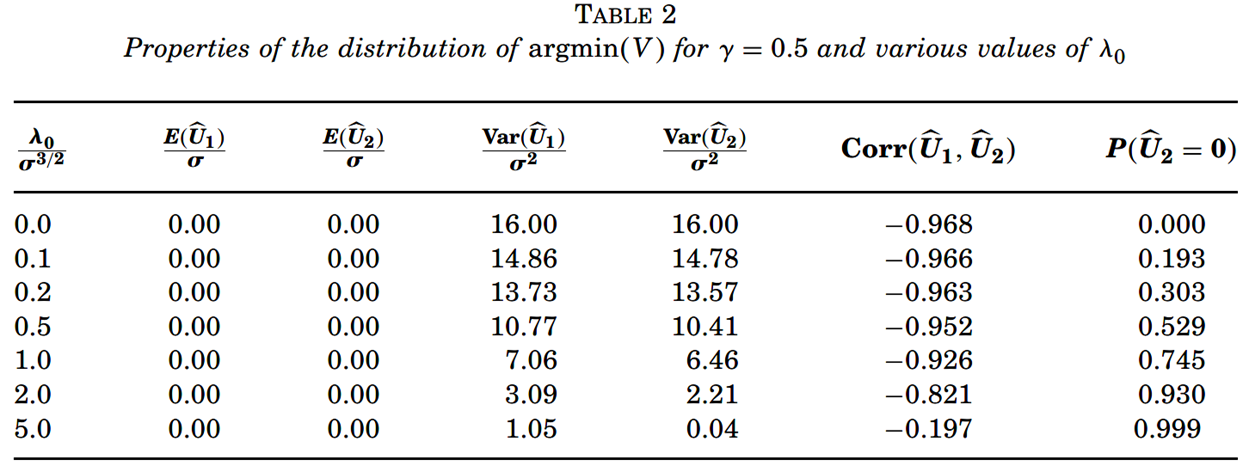
\includegraphics[width=1\linewidth]{image007.png}
		\end{figure}
	\end{frame}
	
	\begin{frame}
		\frametitle{Limiting distributions}
		Scatter plot of random samples (500) from limiting distribution. OLS, $\lambda_0 = 0$
		\begin{figure}
			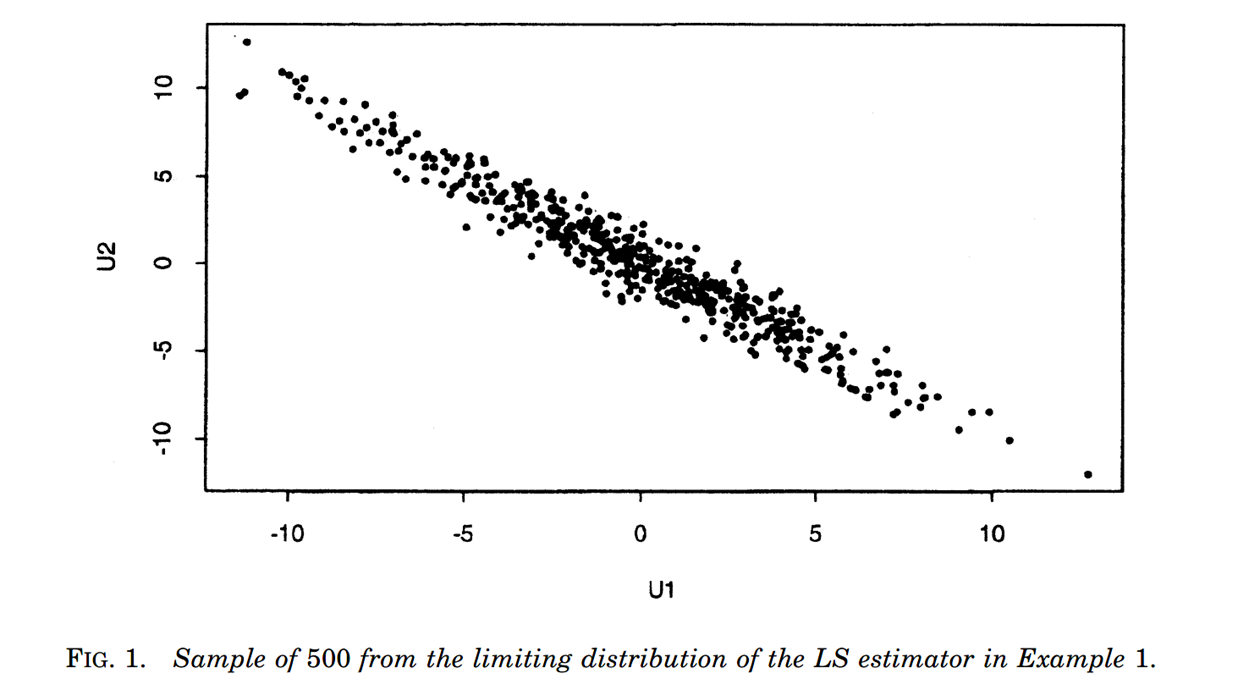
\includegraphics[width=.8\linewidth]{image008.png}
		\end{figure}
		Strong correlation: overestimation of $\beta_1$ always accompanied by underestimation of $\beta_2$ (and vice versa).
	\end{frame}
	
	\begin{frame}
		\frametitle{Limiting distributions}
		LASSO, $\lambda = 1$
		\begin{figure}
			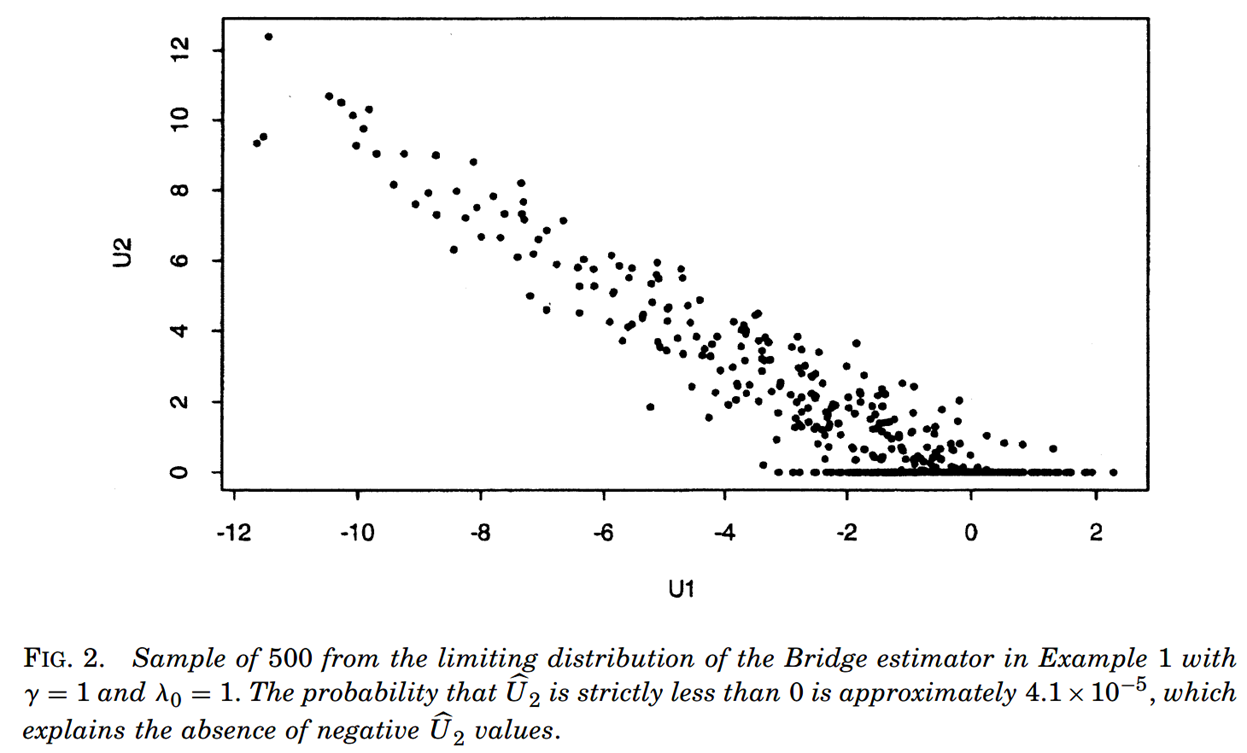
\includegraphics[width=.8\linewidth]{image009.png}
		\end{figure}
		Effectively sets the estimate of $\beta_2$ to 0, if $\beta_1$ is overestimated.
	\end{frame}
	
	\begin{frame}
		\frametitle{Limiting distributions}
		$\lambda = 0.5$
		\begin{figure}
			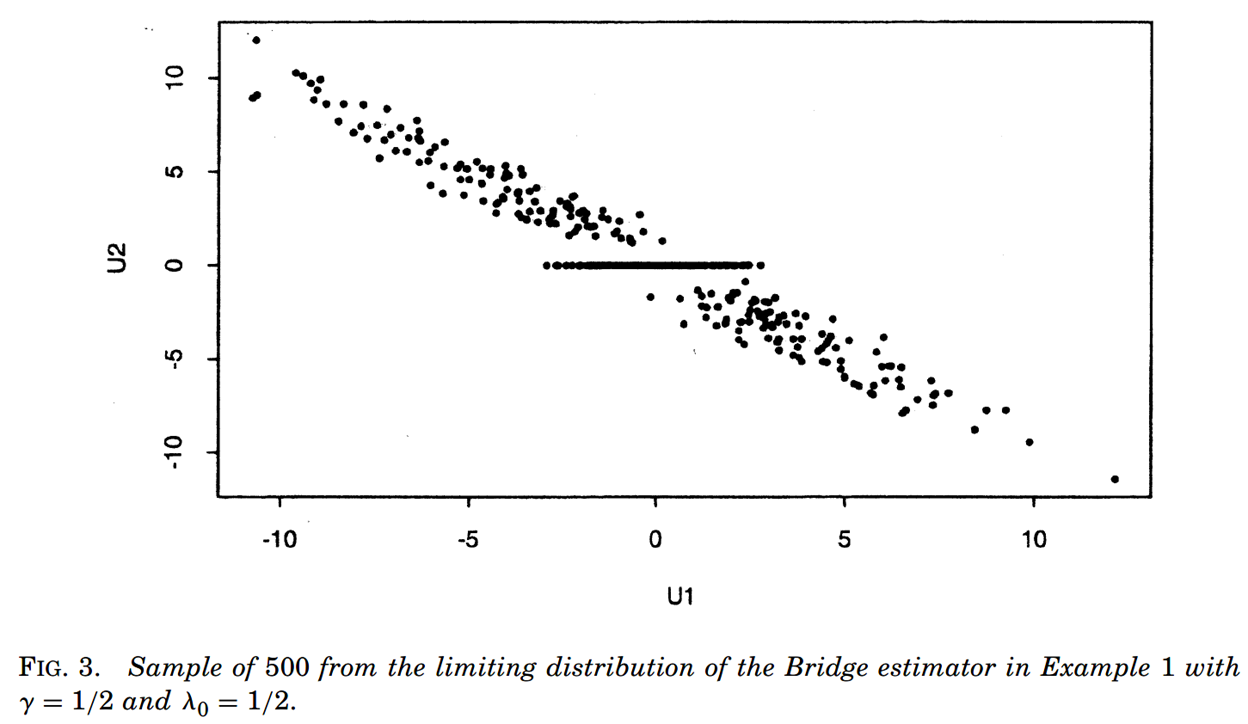
\includegraphics[width=.8\linewidth]{image010.png}
		\end{figure}
		The shrinkage is more selective. And there's a gap in the distribution of $\hat{U}_2$ ("no man's land")
	\end{frame}
	
	\begin{frame}
		\frametitle{Local asymptotics and small parameters}
		They further consider the performance for finite sample. They show how the "exact 0" phenomenon occur in finite samples, when the true parameter is small bu nonzero ($\gamma \leq 1$). The statement \& proofs are similar.
		\begin{figure}
			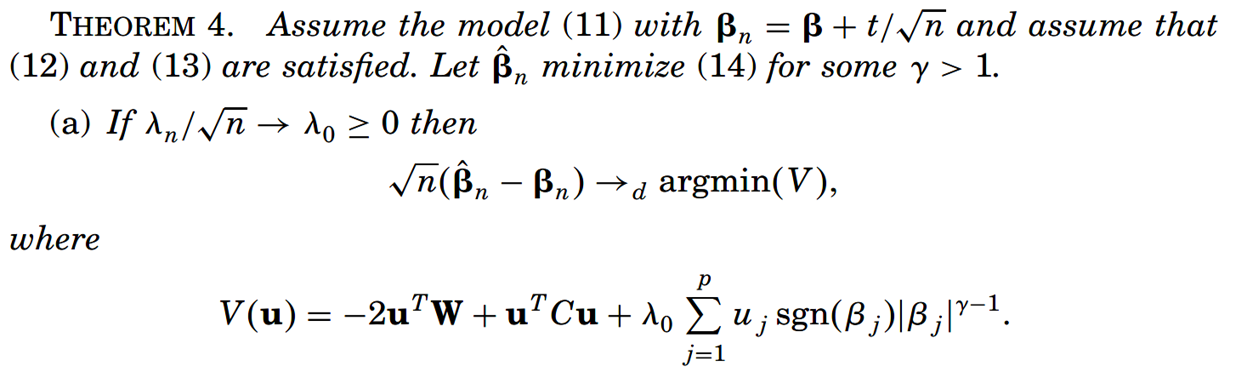
\includegraphics[width=.8\linewidth]{image011.png}
			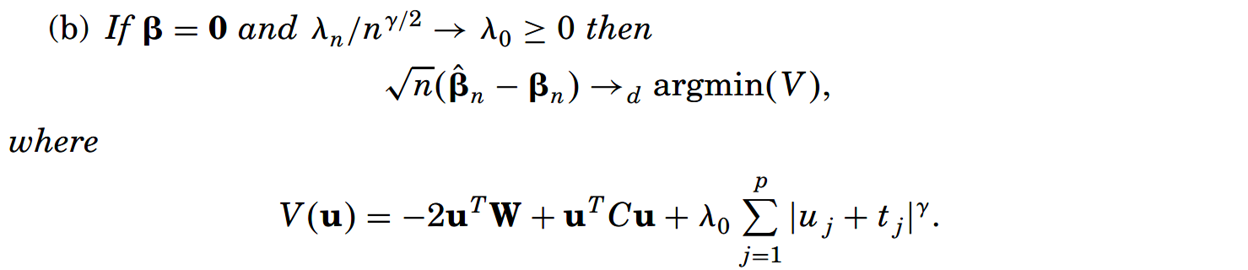
\includegraphics[width=.8\linewidth]{image012.png}
		\end{figure}
	\end{frame}
	
	\begin{frame}
		\frametitle{Local asymptotics and small parameters}
		\begin{figure}
			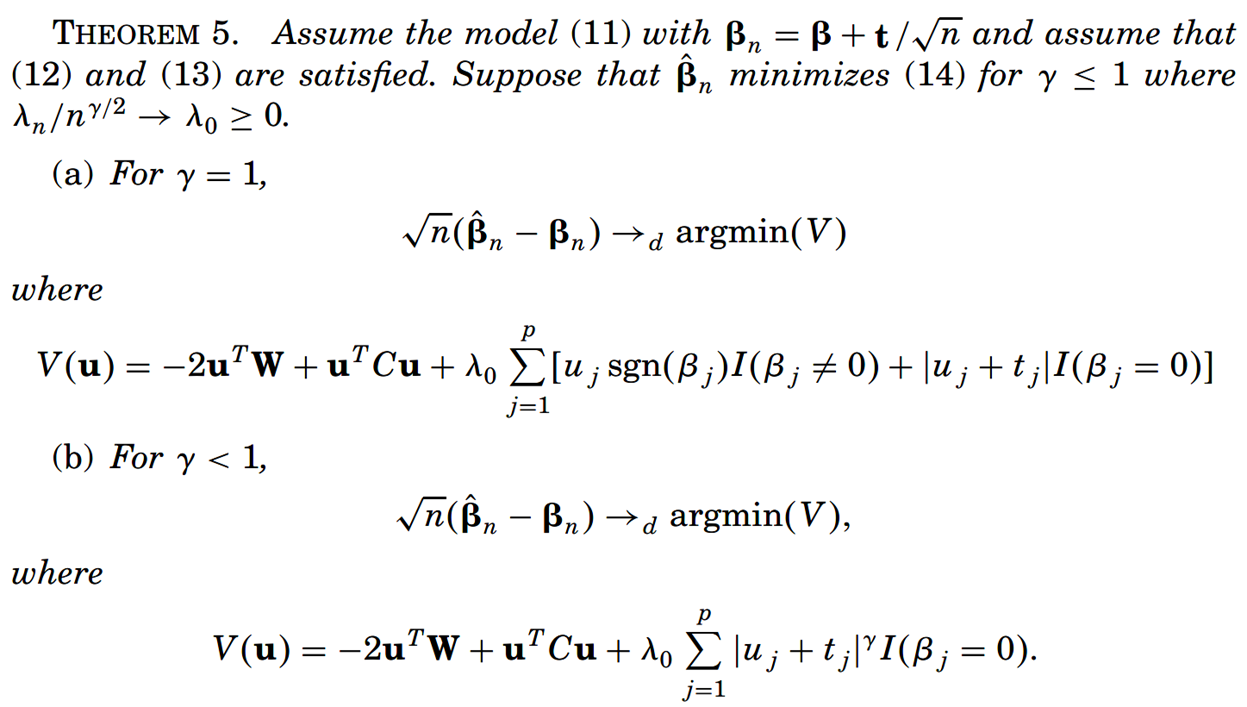
\includegraphics[width=1\linewidth]{image013.png}
		\end{figure}
	\end{frame}
	
	\begin{frame}
		\frametitle{Bootstrapping}
		Estimating the standard error to bridge parameter estimates is nontrivial, especially when $\gamma \leq 1$.
		\vspace{\baselineskip}
		One natural idea is to use bootstrapping. But the asymptotic results show that the bootstrap may introduce bias that doesn't vanish asymptotically, when
		\begin{itemize}
			\item 
			$\gamma < 1$ 
			\item
			some true parameters are either exactly 0 or close to 0.
		\end{itemize}
	\end{frame}
	
	\begin{frame}
		\frametitle{Nearly singular design}
		$$C_n = \frac{1}{n}\sum_{i=1}^{n}\bm{x}_i^T\bm{x}_i \to C$$
		In the last section, they consider the nearly singular design. That is, $C_n$ is not singular, but $C$ is singular.
	\end{frame}
	
	
	\begin{frame}
		\frametitle{Nearly singular design}
		\begin{figure}
			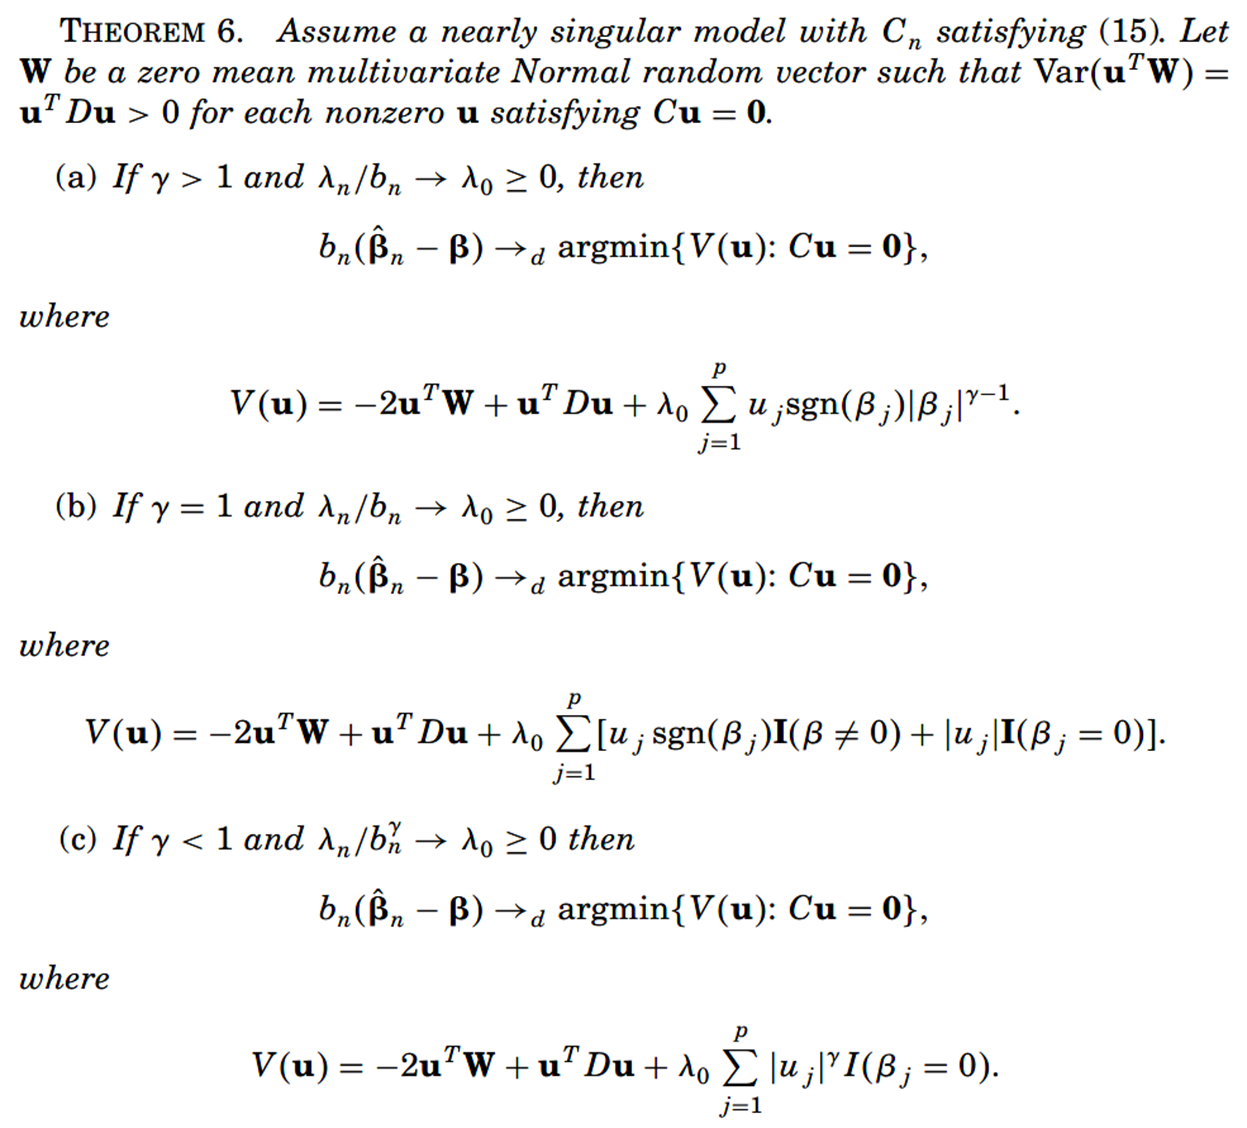
\includegraphics[width=.7\linewidth]{image015.png}
		\end{figure}
	\end{frame}
	
	\begin{frame}
		\frametitle{Nearly singular design}
		One example for nearly singular design...
		\begin{figure}
			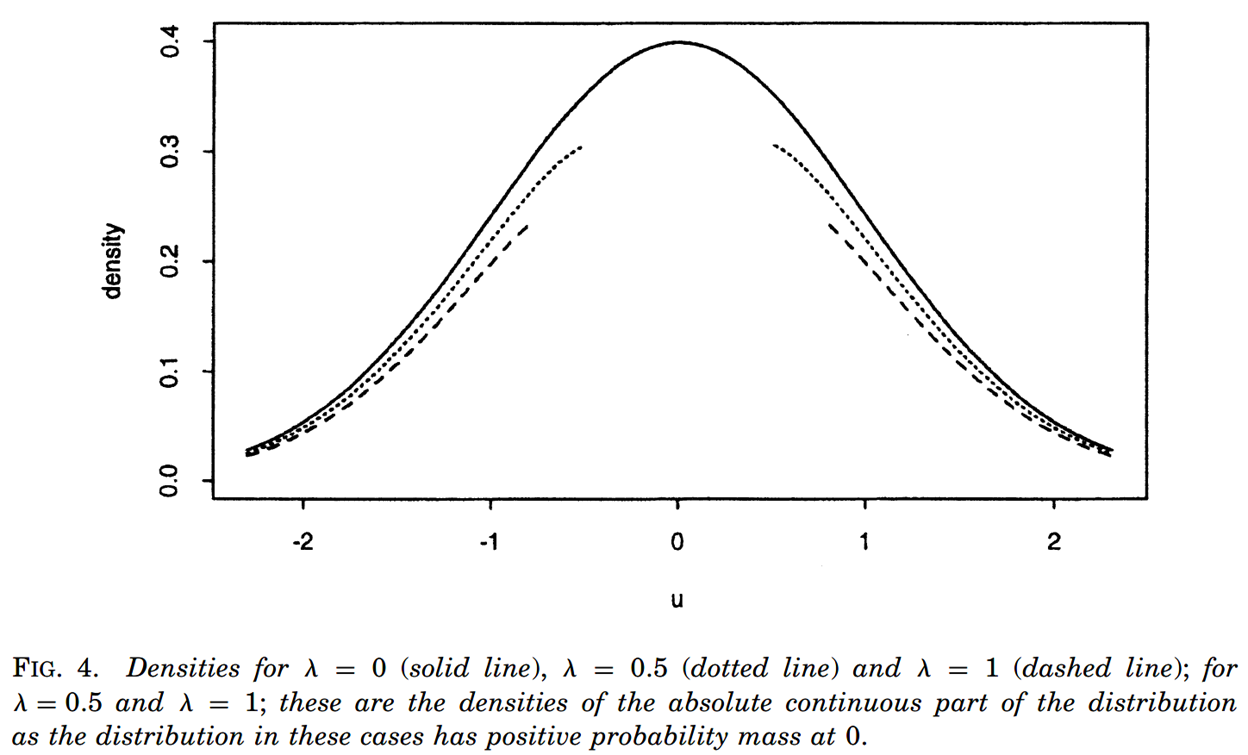
\includegraphics[width=.8\linewidth]{image016.png}
		\end{figure}
		$P(\hat{U} = 0) = 0, 0.448, 0.655$ for $\gamma = 0, 0.5, 1$
	\end{frame}
	
	
	
	
\end{document}